% Digital Logic Report Template
% Created: 2020-01-10, John Miller

%==========================================================
%=========== Document Setup  ==============================

% Formatting defined by class file
\documentclass[11pt]{article}

% ---- Document formatting ----
\usepackage[margin=1in]{geometry}	% Narrower margins
\usepackage{booktabs}				% Nice formatting of tables
\usepackage{graphicx}				% Ability to include graphics

%\setlength\parindent{0pt}	% Do not indent first line of paragraphs 
\usepackage[parfill]{parskip}		% Line space b/w paragraphs
%	parfill option prevents last line of pgrph from being fully justified

% Parskip package adds too much space around titles, fix with this
\RequirePackage{titlesec}
\titlespacing\section{0pt}{8pt plus 4pt minus 2pt}{3pt plus 2pt minus 2pt}
\titlespacing\subsection{0pt}{4pt plus 4pt minus 2pt}{-2pt plus 2pt minus 2pt}
\titlespacing\subsubsection{0pt}{2pt plus 4pt minus 2pt}{-6pt plus 2pt minus 2pt}

% ---- Hyperlinks ----
\usepackage[colorlinks=true,urlcolor=blue]{hyperref}	% For URL's. Automatically links internal references.

% ---- Code listings ----
\usepackage{listings} 					% Nice code layout and inclusion
\usepackage[usenames,dvipsnames]{xcolor}	% Colors (needs to be defined before using colors)

% Define custom colors for listings
\definecolor{listinggray}{gray}{0.98}		% Listings background color
\definecolor{rulegray}{gray}{0.7}			% Listings rule/frame color

% Style for Verilog
\lstdefinestyle{Verilog}{
	language=Verilog,					% Verilog
	backgroundcolor=\color{listinggray},	% light gray background
	rulecolor=\color{blue}, 			% blue frame lines
	frame=tb,							% lines above & below
	linewidth=\columnwidth, 			% set line width
	basicstyle=\small\ttfamily,	% basic font style that is used for the code	
	breaklines=true, 					% allow breaking across columns/pages
	tabsize=3,							% set tab size
	commentstyle=\color{gray},	% comments in italic 
	stringstyle=\upshape,				% strings are printed in normal font
	showspaces=false,					% don't underscore spaces
}

% How to use: \Verilog[listing_options]{file}
\newcommand{\Verilog}[2][]{%
	\lstinputlisting[style=Verilog,#1]{#2}
}




%======================================================
%=========== Body  ====================================
\begin{document}

\title{System on Chip: Class Report 2}
\author{Noel Sengel and John Westbrook}

\maketitle


\section*{Summary}

In this class report, our goal was to create a reaction game using an LED on our NEXYS board. Once the LED lit up, a timer started to see how long it took the person playing to press a button and react. To accomplish this, we took code from a previous class which converted binary to Binary Coded Decimal and displayed it on the 7 segment display. Then, we added our own code and editted the modules to display the millisecond timer while it was running. Our main development occured in one module, "reaction\_timer".


\section*{Results}

Here is a test we did for reaction\_timer module which ensures its functionality
\begin{figure}[ht]\centering
	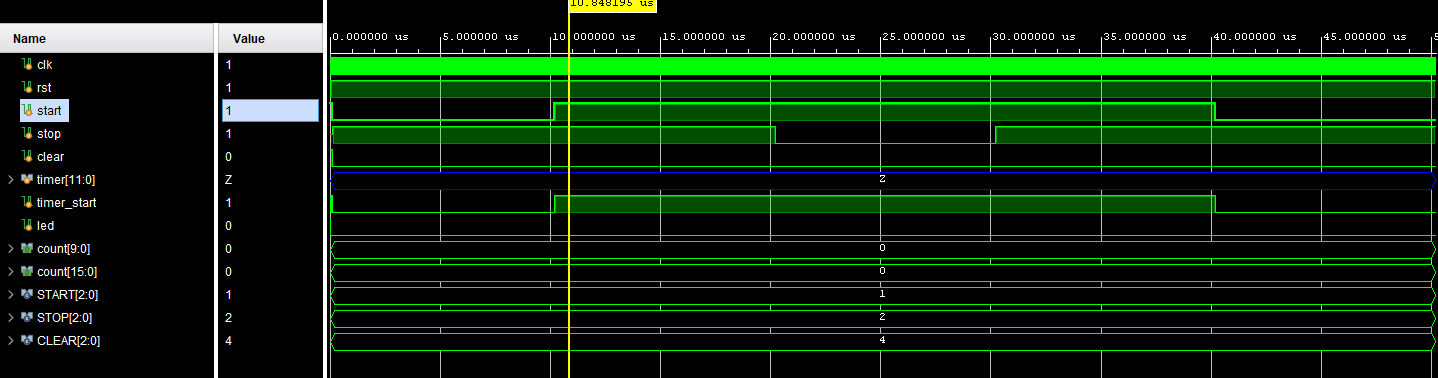
\includegraphics[width=\textwidth]{image_2023-09-14_215312515.png}
	\caption{reaction\_timer Simulation}
	\label{fig1}
\end{figure}

In this GitHub link provided below, there is a video of our board working mostly as desired. As of the writing of this report, we are struggling to have "Hi" displayed before the game starts and some other overflow when pressing the button before the LED goes off.
\section*{Code}

Here is the GitHub repo with our modules: 
\url{https://github.com/JhnWstbrk/ELC4396_ClassReport2}

In Listing 1, you can see a section of our main module, "reaction\_timer", which is the main logic that implements the game part.
\begin{lstlisting}[style=Verilog,
caption=Main Logic of reaction\_timer,
label=code:ex 
]
...
	always_comb begin
	        if(reaction_state == START) begin
	              led = 1'b1;
	              led_on = 1'b1;
	               timer_start = 1'b1;
	        end    
	        if(reaction_state == STOP && timer_start == 1'b1) begin
	             //display last time on the screen
	            timer_start = 1'b0;
	            led = 1'b0;
	        end
	        if(timer == 1000) begin
		        timer_start = 1'b0;
		        led = 1'b0;
		    end
		    
	        if(reaction_state == STOP && led_on != 1'b1) begin
	            
	        end
	        if(reaction_state == CLEAR || rst == 1'b1) begin
	            led = 1'b0;
	            
	        end
	    end
...
\end{lstlisting}


\end{document}
